\chapter{Soluzione proposta}

La soluzione proposta è suddivisa in due fasi principali:
\begin{itemize}
	\item \textbf{Fase 1}: Suddivisione in caratteri
	\item \textbf{Fase 2}: Classificazione del carattere
\end{itemize}

Per la prima fase vengono utilizzati algoritmi di image processing per suddividere la parola in caratteri. Per la seconda fase viene utilizzato un modello di deep learning per classificare i singoli caratteri.

\textcolor{red}{mettere schema pipeline?}

\section{Fase 1: Suddivisione in caratteri}

Come prima cosa, prima di iniziare a suddividere in caratteri l'immagine, vengono effettuate alcune operazioni di pre-processing. In particolare, viene effettuata una normalizzazione dei colori seguita da una binarizzazione dell'immagine.

A questo punto, l'immagine ottenuta è composta da pixel bianchi o neri. Tramite \textcolor{red}{alcune euristiche}, si individua se l'immagine presenta caratteri bianchi su sfondo nero, o viceversa. Essendo la rete allenata su immagini a testo bianco e sfondo nero, l'euristica permette di invertire i colori dell'immagine, se necessario.
\newline

\textcolor{red}{immagini?}

Il primo approccio utilizzato per la suddivisione in caratteri è stato quello di considerare le proiezioni verticali dell'immagine. Come prima cosa si individuano le colonne in cui è presente almeno un pixel bianco.
L'euristica quindi considera due colonne consecutive come appartenenti allo stesso carattere se presentano entrambe almeno un pixel bianco. Nonostante questo approccio possa sembrare ragionevole, gli esperimenti effettuati mostrano non essere efficace per immagini a bassa risoluzione. Infatti, in questo caso, i caratteri tendono a sovrapporsi e le colonne consecutive presentano pixel bianchi in comune. Per questo motivo, si è deciso di utilizzare un approccio alternativo.
\newline

Il secondo approccio utilizzato è quello di considerare le componenti connesse bianche dell'immagine. Questo metodo è più efficace, consentendo di individuare più facilmente caratteri diversi, anche se parzialmente sovrapposti. L'algoritmo non consente di individuare correttamente i caratteri non contigui, come nel caso di `i` e `j`, che presentano un punto sopra il corpo del carattere. Un'ulteriore euristica risolve il problema in maniera efficace, andando a unire due componenti connesse \textcolor{red}{se la distanza tra i loro centri di massa è inferiore a una certa soglia}. In questo modo, si riesce a ottenere un'immagine in cui ogni carattere è rappresentato da una singola componente connessa.
\newline

Una volta individuati i bounding box dei caratteri, si procede anche a calcolare un bounding box globale che racchiude tutti i caratteri. L'utilità di questo bounding box viene mostrata nella fase di classificazione.

\begin{figure}[H]
	\centering
	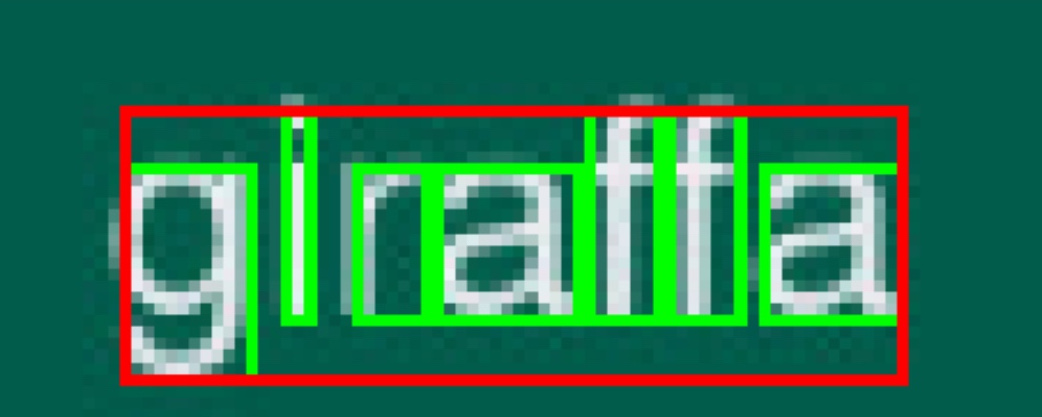
\includegraphics[width=0.3\textwidth]{images/giraffa-bb.jpeg}
	\caption{Individuazione Bounding Box}
	\label{fig:screenshot}
\end{figure}

\section{Fase 2: Classificazione del carattere}

Per la classificazione del carattere viene utilizzato un modello di deep learning. \textcolor{red}{Il modello è una CNN (Convolutional Neural Network) che è stata allenata su un dataset di immagini di caratteri.}
Il modello lavora su immagini di dimensioni 28x28 pixel, quindi è necessario ridimensionare i caratteri estratti dalla fase 1.


Passando al modello esclusivamente il carattere ridimensionato, di quest'ultimo verrebbero ignorate la dimensione e la posizione all'interno della parola. Questa semplificazione causerebbe problemi nella classificazione della punteggiatura e di caratteri \emph{confondibili}.

Senza informazioni sulla posizione, il modello non sarebbe in grado di distinguere tra `,` e `'`. Inoltre, non sarebbe in grado di distinguere tra maiuscole e minuscole \emph{confondibili}.
\newline

Per carattere \emph{confondibile} si intende una lettera in cui la rappresentazione in stampatello minuscolo coincide con quella in stampatello maiuscolo, se ridimensionata. Ad esempio, `C` e `c` sono caratteri confondibili, così come `S` e `s`, mentre `A` e `a` non lo sono.
L'insieme dei caratteri confondibili maiuscoli ($\text{CI}$) è definito come segue:
$$\text{CI} = \{C, J, K, O, P, S, U, V, W, X, Z\}$$

Ovviamente la controparte minuscola contiene gli stessi caratteri.

\subsection{Utilizzo del Bounding Box globale}

È possibile utilizzare il bounding box globale per fornire al modello informazioni sulla posizione e la dimensione del carattere all'interno della parola. Partendo dal bounding box del carattere e da quello globale, è possibile estrarre il margine superiore e inferiore del carattere rispetto al bounding box globale. Una volta normalizzati rispetto all'altezza del bounding box globale, il margine superiore e inferiore del carattere possono essere utilizzati come due parametri aggiuntivi per il modello.

Con questo accorgimento, il modello è adesso in grado distinguere tra `,` e `'`. Inoltre, nel caso della parola `Bob`, è in grado di classificare correttamente la `o`. Questo è possibile in quanto il margine superiore della `o` è solo presente nel caso in cui il carattere sia maiuscolo.

\subsection{La necessità di euristiche}

Nonostante quest'ultimo approccio possa sembrare efficace, non è sempre in grado di distinguere tra maiuscole e minuscole.
Mostriamo il motivo attraverso un esempio e lo formalizziamo successivamente.
Consideriamo due parole d'esempio:
\begin{itemize}
	\item `Cocco`: la prima lettera non ha margine superiore e inferiore, e deve essere classificata come maiuscola.
	\item `cocco': la prima lettera non ha margine superiore e inferiore, e deve essere classificata come minuscola.
\end{itemize}

Il modello non è quindi in grado di classificare correttamente i caratteri confondibili quando hanno la stessa altezza del bounding box globale.
È necessario utilizzare un'euristica che, confrontando l'altezza dei vari caratteri, sia in grado di `correggere` la forma maiuscola o minuscola del carattere.

Guardando la distribuzione dei caratteri rispetto al loro margine superiore, è possibile notare quando è possibile classificare con certezza i caratteri confondibili.

\begin{figure}[H]
	\centering
	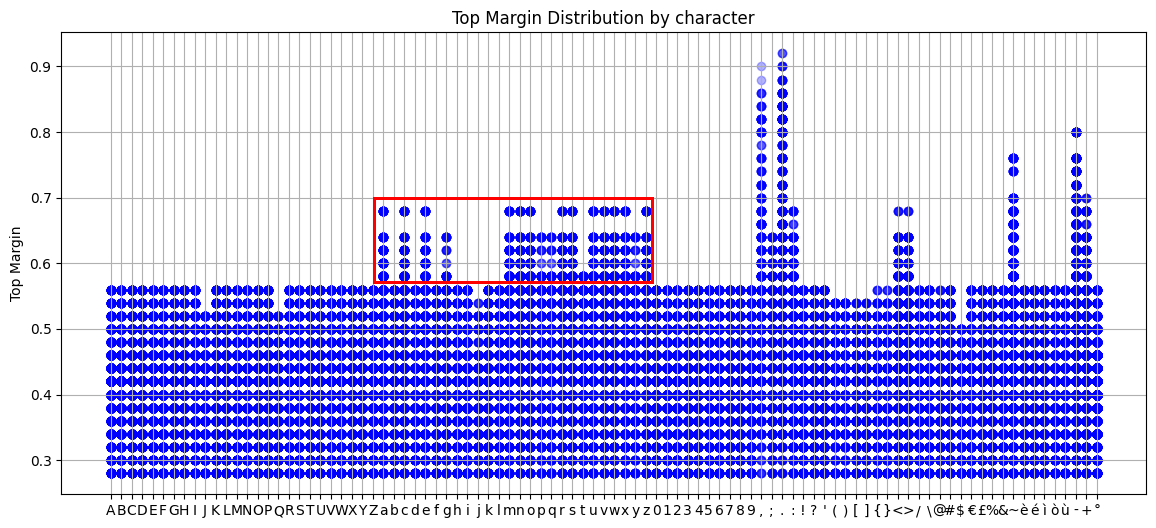
\includegraphics[width=1\textwidth]{images/top_margin_distribution_highlight.png}
	\caption{Distribuzione dei caratteri rispetto al margine superiore. Il rettangolo rosso evidenzia i caratteri confondibili identificabili con affidabilità.}
	\label{fig:top_margin_distribution_highlight.png}
\end{figure}

Rimane comunque il fatto che parole come `COCCO' e `cocco' rimangono indistinguibili anche all'occhio umano, se non affiancate da altre parole che possano disambiguare.

\subsection{L'applicazione dell'euristica}

Data una determinata immagine, per carattere \emph{affidabile} intendiamo un carattere non confondibile oppure un carattere confondibile di forma minuscola con margine superiore significativo. Un carattere è quindi affidabile quando la sua interpretazione agli occhi del modello è priva di ambiguità.

L'euristica dev'essere applicata quando è presente un carattere confondibile la cui altezza coincide con quella del bounding box globale. In questo caso, l'euristica confronta l'altezza del carattere con quella degli altri caratteri affidabili della parola.
L'unico caso in cui l'altezza di un carattere confondibile coincide con quella del bounding box globale è quando non sono presenti caratteri che aumentano l'altezza del bounding box globale. Tra questi sono inclusi tutti i caratteri maiuscoli e qualche carattere minuscolo, come `b`, `d` e `h`.
